%%%%%%%%%%%%%%%%%%%%%%%%%%%%%%%%%%%%%%%%%
% Journal Article
% LaTeX Template
% Version 1.3 (9/9/13)
%
% This template has been downloaded from:
% http://www.LaTeXTemplates.com
%
% Original author:
% Frits Wenneker (http://www.howtotex.com)
%
% License:
% CC BY-NC-SA 3.0 (http://creativecommons.org/licenses/by-nc-sa/3.0/)
%
%%%%%%%%%%%%%%%%%%%%%%%%%%%%%%%%%%%%%%%%%

%----------------------------------------------------------------------------------------
%	PACKAGES AND OTHER DOCUMENT CONFIGURATIONS
%----------------------------------------------------------------------------------------

\documentclass[twoside]{article}

%\usepackage{wrapfig}

\usepackage[sc]{mathpazo} % Use the Palatino font
\usepackage[T1]{fontenc} % Use 8-bit encoding that has 256 glyphs
\linespread{1.05} % Line spacing - Palatino needs more space between lines
\usepackage{microtype} % Slightly tweak font spacing for aesthetics
\usepackage{graphicx}
%\usepackage{subfig} % make it possible to include more than one captioned figure/table in a
%\graphicspath{ {images/} }
%\graphicspath{ {figures/} }

\usepackage[hmarginratio=1:1,top=32mm,columnsep=20pt]{geometry} % Document margins
\usepackage{multicol} % Used for the two-column layout of the document
\usepackage[hang, small,labelfont=bf,up,textfont=it,up]{caption} % Custom captions under/above floats in tables or figures
\usepackage{booktabs} % Horizontal rules in tables
\usepackage{float} % Required for tables and figures in the multi-column environment - they need to be placed in specific locations with the [H] (e.g. \begin{table}[H])
\usepackage{hyperref} % For hyperlinks in the PDF

\usepackage{lettrine} % The lettrine is the first enlarged letter at the beginning of the text
\usepackage{paralist} % Used for the compactitem environment which makes bullet points with less space between them

\usepackage{abstract} % Allows abstract customization
\renewcommand{\abstractnamefont}{\normalfont\bfseries} % Set the "Abstract" text to bold
\renewcommand{\abstracttextfont}{\normalfont\small\itshape} % Set the abstract itself to small italic text

\usepackage{titlesec} % Allows customization of titles
\renewcommand\thesection{\Roman{section}} % Roman numerals for the sections
\renewcommand\thesubsection{\Roman{subsection}} % Roman numerals for subsections
\titleformat{\section}[block]{\large\scshape\centering}{\thesection.}{1em}{} % Change the look of the section titles
\titleformat{\subsection}[block]{\large}{\thesubsection.}{1em}{} % Change the look of the section titles

\usepackage{fancyhdr} % Headers and footers
\pagestyle{fancy} % All pages have headers and footers
\fancyhead{} % Blank out the default header
\fancyfoot{} % Blank out the default footer
%%AH\fancyhead[C]{Running title $\bullet$ November 2012 $\bullet$ Vol. XXI, No. 1} % Custom header text
%%\fancyhead[C]{November 18th, 2014}
\fancyfoot[RO,LE]{\thepage} % Custom footer text

%----------------------------------------------------------------------------------------
%	TITLE SECTION
%----------------------------------------------------------------------------------------

\title{\vspace{-15mm}\fontsize{24pt}{10pt}\selectfont\textbf{Hadoop Poker: Machine Learning in Texas Hold'em}} % Article title

\author{
\large
\textsc{Adrienne Humblet, David Kasofsky}\\[2mm] 
\normalsize New York University \\ 
\date{}
\vspace{-5mm}
}


%----------------------------------------------------------------------------------------

\begin{document}

\maketitle{} % Insert title

\thispagestyle{fancy} % All pages have headers and footers

%----------------------------------------------------------------------------------------
%	ABSTRACT
%----------------------------------------------------------------------------------------

\begin{abstract}

\noindent {
No Limit Hold 'Em (NLHE) is a fun recreational game for many around the world and a TV sensation. This project develops a tool for analyzing the simplest decisions in NLHE, namely when the player when has opportunity to make the first move in a hand. We use hand histories, i.e. the logs of game actions in poker, to train SVMs to classify poker situations. This tool helps players answer the question:''Should I play this hand?''
} 

\end{abstract}

%----------------------------------------------------------------------------------------
%	ARTICLE CONTENTS
%----------------------------------------------------------------------------------------

\begin{multicols}{2} % Two-column layout throughout the main article text

\section{Introduction}
An online poker site, e.g. PokerStars.com will easily play billions of hands per year and a professional poker player may play hundreds of thousands if not millions of hands per year. Each of these hands is logged as part of what is called a hand history.
We acquired hand histories to analyze in Hadoop with the intention of developing poker strategy guidelines. Our sources were 10 months of hand histories from a professional poker player and 7 years of hand histories from an IRC poker channel.
We focused on one of the most popular forms of poker: No Limit Texas Hold 'Em (NHLE) tournaments. One can find a detailed description at \cite{TexasHoldem}. Poker hands vary significantly in their complexity so we limited ourselves to the cases in which a player has the opportunity to make the first bet and is not in the blinds. We created feature vector representations of these situations, generated summary statistics, and used support vector machines (SVMs) to predict when a player should play or fold a hand, using the professional player's hand history as the bar for good performance.

%------------------------------------------------

\section{Motivation}

Poker is an interesting game to study for several reasons. First, it is a multi-billion dollar industry, e.g. PokerStars.com was purchased for almost \$5 billion in 2014 \cite{PokerStarsAcquired} and is only one of hundreds of online poker sites. Second, it is a classical game of logic, deception and mathematics, requiring a basic knowledge of probability and game theory. Third, many consider poker a model game for the development of machine learning, such as the University of Alberta Computer Poker Research Group (CPRG) \cite{SVMPoker}. There is much analysis surrounding poker academically, e.g. CPRG, and commercially, e.g. analytical poker software like Poker Tracker \cite{PokerTracker}. In particular, NLHE tournament poker is the most popular form of poker. It is the format for the World Series of Poker Main Event, the most prestigious poker tournament in the world. 

%------------------------------------------------

\section{Related Work}

The CPRG has published many papers related to our topic.
One such paper \cite{SVMPoker} describes using a support vector machine to train a poker bot on post-flop strategy. Since this yielded effective results, our project aims to extend a similar SVM mechanism for pre-flop strategy.

Others, such as \cite{holdemml}, have used machine learning to build poker bots. SVMs and other classification algorithms are used to select an action to take based on a given situation.

None of the research we encountered focused the the simple situations we have chosen to analyze.

%------------------------------------------------

\section{Design}

\subsection{Data Sources}
We used two sources of hand histories.
\begin{compactitem}
\item{PokerStars Hand History} - Our first source is the private hand history of professional poker player Jaime Staples who kindly agreed to donate his data to us. Jaime Staples is a 23 year old Canadian with six figures of NLHE tournament cashes \cite{JaimeStaples} and is sponsored by PokerStars. This hand history is about 700MB of raw data.
\item{IRC Poker Database} - Our second source is seven years of poker data scraped from a dozen IRC poker channels. It was compiled and made available by the CPRG \cite{IRCDatabase}. 
We only used the data from the no limit hold'em and  no limit hold'em tournament channels, resulting in 3.8 million poker hands (876MB of raw data). 
\end{compactitem}

\subsection{Labels and Feature Vectors}

Our feature vectors consist of 12 features: \newline
\indent - number of players in the hand\newline
\indent - player's position \newline
\indent - players' stacks \newline
\indent - player's hand strength \newline

The associated label was then either 1 (Play) or 0 (Fold) depending on the action taken by the player in question. We designed the feature vectors in this way since this represents the basic information available to a player, i.e. the feature vectors are from a single player's perspective and so we only know that player's cards. Call this player the active player. Thus the position and hand strength features are with respect to the active player. We can use this representation because we have restricted ourselves to situations in which no other player has bet or raised before the player in question. This means that players in earlier position have all folded and so we do not need to account for other actions. If we did not limit ourselves to this case, our analysis would become much more complicated and these features would likely be inadequate. We will discuss this further in our Future Work section.

The feature vectors were normalized in a slightly peculiar way due to the nature of the data. The number of players was normalized by division by 9 as there at most 9 players in a hand. The player's position is the clockwise distance from the button, which ranges from 0 to 8 and was normalized by division by 8. The players' stacks (numbers of chips) are in clockwise order around the table starting with the player in question and are normalized by division by the largest stack. Hand strength is the probability that the active player's hand wins against a single random hand and so lies between 0 and 1.

One of our biggest challenges was finding a feature vector that was possible based to produce from both of our datasets. For instance, Jaime Staples' hands contained which cards he was dealt at the beginning of the hand and so the active player's cards were known regardless of the outcome. However the IRC hands are recorded by an observer and so a player's hand is only revealed if it is revealed at showdown at the conclusion of the hand. Thus we could only retrieve positive examples (if the active player chose to play the hand as opposed to fold) from the IRC data since if the player folded at any point then their hand would never be revealed to the observer. Similarly the Jamie Staples data contained all information about a hand whereas the IRC data only showed summary information about the hand's conclusion. Another concern is while Jamie Staples is a successful professional \cite{JaimeStaples} the IRC database provided no guarantee about the skill levels of the players.

In light of these limitations as well as the complexity in developing a comprehensive analysis of poker strategy, we confined ourselves to the simplest poker situations described previously, in which the active player has the opportunity to make the first bet and is not in the blinds. It is a bit of a special case when a player is in the blinds and so chose to ignore these hands for simplicity's sake. As an example, consider the following sequence of actions:\\
\indent Position 1 - big blind\\
\indent Position 2 - little blind\\
\indent Position 3 - fold\\
\indent Position 4 - fold\\
\indent Position 5 - fold\\
\indent Position 6 - call\\
\indent Position 7 - raise\\
\indent Position 8 - call\\
\indent Position 9 - fold\\
If the active player was in position 3, 4, 5, or 6 then we would use the hand. Positions 3, 4, and 5 fulfill our criteria because the player has the opportunity to make the first bet even though they choose to fold. Position 6 also fulfills our criteria because the play makes the first bet. A bet has been made (by the player in position 6) before the players in positions 7,8, and 9 have had a chance to bet and so these situations would be excluded. Positions 1 and 2 are always excluded because they correspond to the blinds.

\subsection{Map Reduce Jobs}

\begin{figure}[H]
  \centering
  \centerline{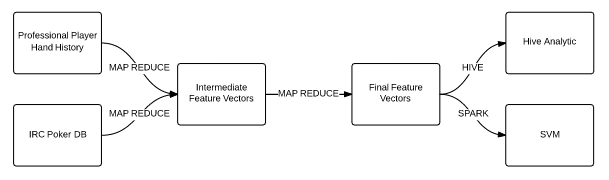
\includegraphics[width=0.5\columnwidth]{Flowchart.png}}
   \caption{Data Flowchart}
  \label{fig:Data flow}
\end{figure}

Using MapReduce, we extracted feature vectors from both data sets and merged them. At this point we the hand strength feature was simply the string representation of the cards, e.g. AsKs for the Ace of Spades and the King of Spades. Next, we ran the combined dataset into another MapReduce that translated the string hand representation into the probability that it wins against a single random hand. We used the resulting final feature vectors set to train SVMs using Spark and to summarize and analyze the data using Hive. 

%------------------------------------------------

\section{Results}

\subsection{Position and hand strength}

By manipulating the data in Hive, we noticed a clear relationship between position, hand strength, and whether to fold or play a hand. Figure 2 shows all of our cleaned data organized by position and hand strength. There are 2 clear observations to be made about our data as a whole: there are significantly more folds than plays and there are fewer of both in the higher positions. Both of these observations, however, are artifacts of our data collection and do not reflect poker strategy. As in the example above, it is possible for one hand of poker data to yield several feature vectors for folding but only one for calling or raising. This explains the larger amount of folding data. And since we only sought to analyze first to act, there is a higher probability of actions occurring in the early positions rather than the latest. This explains the decreasing amount of data as position increases.

\begin{figure}[H]
  \centering
  \centerline{\includegraphics[width=1.1\columnwidth]{Allhands.png}}
   \caption{All Hands}
  \label{fig:allHands}
\end{figure}

To further analyze our data, we divided all the feature vectors by hand strength deciles ranging from 3 to 9 where 3 represents bad cards (e.g. 4 of hearts and 2 of spades) and 9 represents promising cards (e.g. Ace and King of the same suit). Figure\ref{fig:9thDecile} clearly shows that cards in the 9th decile should never be folded. Out of the 1395 hands displayed, only one was folded in pos 7. This results in a .0007\% fold rate across all positions. 

\begin{figure}[H]
  \centering
  \centerline{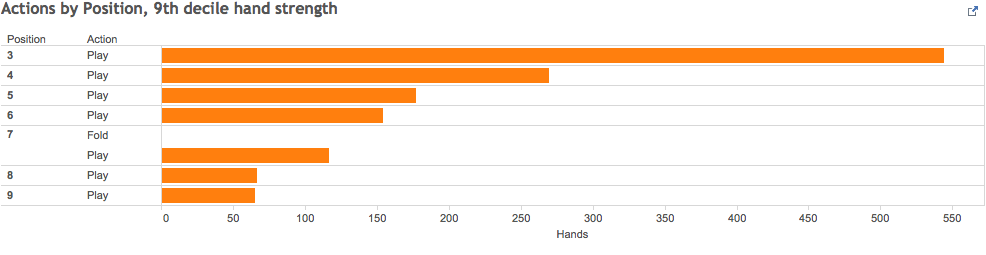
\includegraphics[width=1.1\columnwidth]{9thDecile.png}}
   \caption{9th Decile}
  \label{fig:9thDecile}
\end{figure}

On the opposite end of the spectrum, the 3rd decile is the worst range of card strengths. We expected figure\ref{fig:3rdDecile} to show entirely folds, thus representing the exact opposite of figure\ref{fig:9thDecile}. Instead, we noticed average of 0.014\% total play rate, even among these worst cards. This, we suspect, is the player intentionally misleading the others so their actions don't become too predictable. The need to do this decreases almost linearly as the position increases, starting with 0.026\% play rate at position 3 down to 0.008\% in position 9. 

\begin{figure}[H]
  \centering
  \centerline{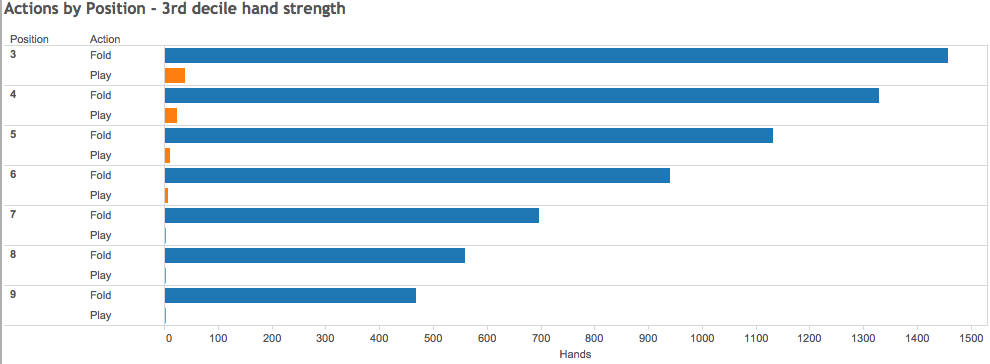
\includegraphics[width=1.1\columnwidth]{3rdDecile.png}}
   \caption{3rd Decile}
  \label{fig:3rdDecile}
\end{figure}

In the middle of the hand strength spectrum, figures \ref{fig:4thDecile}, \ref{fig:5thDecile}, \ref{fig:6thDecile} show the transition from mostly folds to mostly plays. As demonstrated in the figures, the lower positions consistently have a higher fold rate than the higher positions. This is because players with higher positions have already had a chance to gauge the other players' confidences in their hands and with strategic betting can win with a larger range of hand strengths. 

\begin{figure}[H]
  \centering
  \centerline{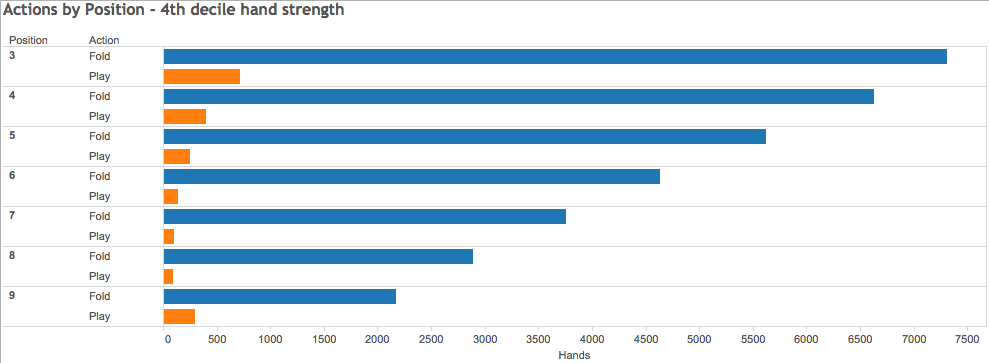
\includegraphics[width=1.1\columnwidth]{4thDecile.png}}
   \caption{4th Decile}
  \label{fig:4thDecile}
\end{figure}

\begin{figure}[H]
  \centering
  \centerline{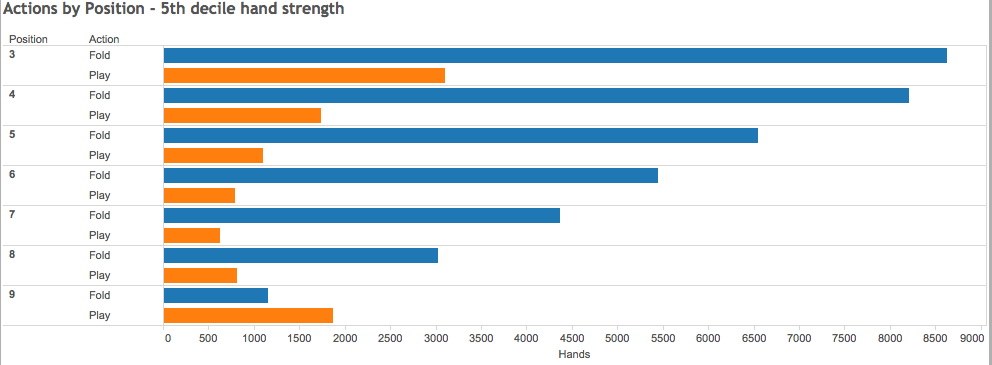
\includegraphics[width=1.1\columnwidth]{5thDecile.png}}
   \caption{5th Decile}
  \label{fig:5thDecile}
\end{figure}

\begin{figure}[H]
  \centering
  \centerline{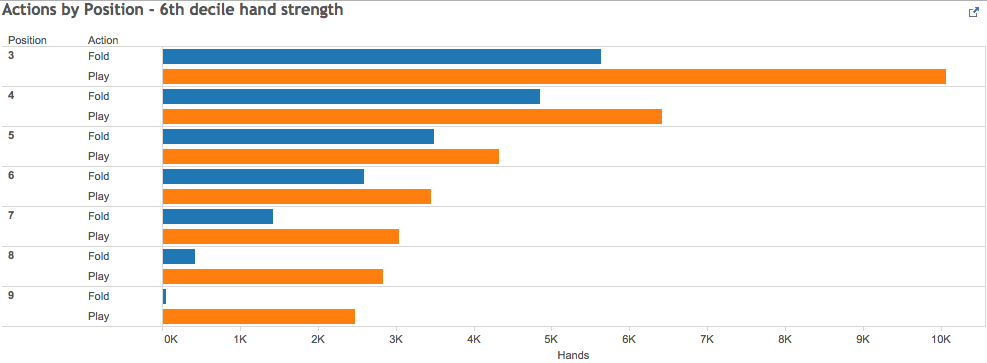
\includegraphics[width=1.1\columnwidth]{6thDecile.png}}
   \caption{6th Decile}
  \label{fig:6thDecile}
\end{figure}

\subsection{Support Vector Machines}

We used Spark to train linear and second degree polynomial kernel SVMs to do binary classification of feature vectors, the two classes being Play (1) and Fold(0). We ranged the regularization parameter $\lambda$ between all odd powers of $2$ between $2^-31$ and $2^3$. The SVM algorithm in Spark uses stochastic gradient descent (SGD). Each SVM was trained 50 iterations of SGD with step size 1 and using the entire sample for each mini-batch. These are the usual parameters of SGD that determine how many examples are used to compute the gradient at each iteration (mini-batch size) and how far to move in the direction of the gradient (step size) before computing it again in the next iteration. We established this range experimentally which suggested that there would be little change in training error outside outside this range. Our best training errors were with small $\lambda$ although none were excellent.

The linear SVM performed best with very little regularization and the degree two polynomial kernel performed best with medium regularization, relatively speaking. Both performed poorly with large regularization. However our results are encouraging since we did manage to have some improvement over random guessing with very simple features. The feature space for the linear SVM is the same as feature vectors described previously and only has dimension 12. The polynomial kernel had dimension 23 features which is still relatively low and could be much, much larger for poker games. See figure \ref{fig:SVM} for a graphical comparison of the linear and polynomial kernel SVM training error.

\begin{figure}[H]
  \centering
  \centerline{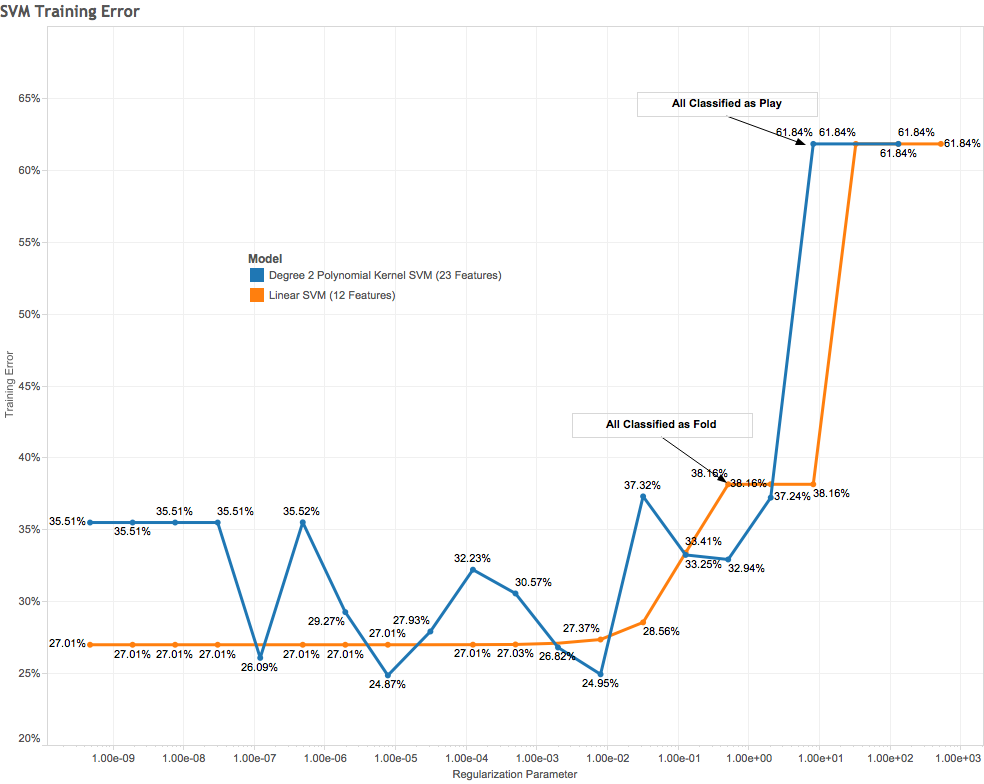
\includegraphics[width=1\columnwidth]{SVM.png}}
   \caption{SVM Training Error}
  \label{fig:SVM}
\end{figure}

%--------------------------------------------

\section{Future Work}

This work could be improved in several ways. First, we could use a far larger poker data set of hand histories by professional players. Even though Jaime's hands numbered in the hundreds of thousands, we could have analyzed many more. This data was better for our purposes since the hands were played by a successful professional and they contained both positive and negative examples, whereas the data from IRC contained only positive examples and the players themselves were of dubious quality. We could also design richer features. We chose a simple feature set here as a starting point, but we may be able to have much better classification results if we had better features. Similarly we could improve the SVM work with the existing features by experimenting with other more complex kernels. We could also compare the SVM results with other classification algorithms such as logistic regression or k-nearest neighbor.

%------------------------------------------------

\section{Conclusion}

Our data revealed several fundamental poker strategies when the player has the opportunity to make the first bet and is not in the blinds:
\begin{compactitem}
\item{} Always play the best hands, e.g. those in the 7th, 8th, and 9th deciles, regardless of position. 
\item{} Almost always fold the worst hands, e.g. those in the 3rd and 4th deciles, especially in the lower positions.
\item{}Be more conservative with hand strength in the early positions. For example, sample hands in 6th hand strength decile were played 64\% of the time in the 3rd position but 98\% of the time in 9th position.
\end{compactitem}
Furthermore, our results were encouraging in designing classifiers than can predict the correct actions to take in NLHE poker tournaments since we were able to do better than random using both modest features and modest number of examples. This project was an excellent exercise in utilizing technologies from the Hadoop ecosystem as well as in thinking about poker strategy.


%------------------------------------------------

\section{Acknowledgements}

Many thanks to Jaime Staples for sending us his hand histories, to the University of Alberta Poker Group for collecting the IRC data, and the NYU HPC for assistance with Spark on Dumbo. 


%----------------------------------------------------------------------------------------
%	REFERENCE LIST
%----------------------------------------------------------------------------------------

\begin{thebibliography}{99} % Bibliography - this is intentionally simple in this template

\bibitem{PokerStarsAcquired} Vardi, Nathan. Amaya Gaming In Geal To Buy PokerStars For \$4.9 Billion. Forbes. Retreived 13 June 2014. 

\bibitem{PokerTracker} Poker Tracker 4 Review. Pokersoftware.com Retrieved 2012-08-26.

\bibitem{JaimeStaples} Jaime Staples Poker Results and Statistics. Official Poker Rankings. Retreived 2015-09-08.

\bibitem{IRCDatabase} Michael Maurer's IRC Poker Database. Retreived 12-8-2015.
\url{http://poker.cs.ualberta.ca/irc_poker_database.html}

\bibitem{TexasHoldem} Wikipedia. Retreived 12-8-2015.
\url{https://en.wikipedia.org/wiki/Texas_hold_%27em}

\bibitem{SVMPoker} J Pfund. Support Vector Machines in the Machine Learning: Classifier for a Texas Hold'em Poker Bot.  University of Pennsylvania, 2007.

\bibitem{clustering} N. Bard, D. Nicholas, C. Szepesvári, and M. Bowling. Decision-theoretic Clustering of Strategies. University of Alberta. 2015

\bibitem{holdemml} L Teofilo, L Reis. HoldemML: A Framework to generate No Limit Hold’em Poker Agents from Human Player Strategies. Conferencia Iberica de Sistemas Tecnologia de Informacao. 2011.

\bibitem{aymmsetric abstractions} N Bard, M Johanson, M Bowling. Asymmetric Abstractions for Adversarial Settings. Proceedings of the Thirteenth International Conference on Autonomous Agents and Multi-Agent Systems (AAMAS). May 2014.
\end{thebibliography}

%----------------------------------------------------------------------------------------

\end{multicols}

\end{document}
